\documentclass[12pt]{article}
\usepackage{amsmath,amsfonts,amssymb,graphicx}
\usepackage{xcolor}
\usepackage{hyperref}
\usepackage{float}
\usepackage{biblatex}
\addbibresource{bibtex.bib}

\usepackage{geometry}
\geometry{a4paper, margin=1in}
\title{Report on Data  Analysis Master Class  - Asteroseismology}
\author{Ema Salugová \& S.M.Masruk Uddin}
\date{January 2025}
\date{}

\begin{document}
\maketitle
\tableofcontents
\section{Introduction}
Asteroseismology is a field of studying the frequency oscillations of the photosphere caused by the sound waves travelling in stelar interiors. Observations of flux or radial velocity variations as a results of these oscillations lead to the power spectrum density (PSD) of the time series. Asteroseismology can reveal information on stellar properties such as mass, radius and age. There are several modes that can be excited. Main two categories are radial and non-radial modes. We differentiate them by their spherical harmonic angular degree, $l$, azimuthal order, $m$, and a radial order, $n$. The essential asteroseismologic quantities are the frequency spacing $\delta \nu$, of the mode peaks and the frequency of maximum power, $\nu_{max}$.

\subsection*{Markov Chains Monte Carlo MCMC}
Markov Chain Monte Carlo (MCMC) methods have become indispensable tools in modern astronomy, enabling researchers to tackle complex problems involving large parameter spaces and high-dimensional data. At its core, MCMC combines the concepts of Markov chains and Monte Carlo integration to efficiently sample from probability distributions, often in the context of Bayesian inference. This introduction outlines the mathematical foundation of MCMC and highlights its applications in astronomical research.

\subsubsection*{Bayesian Inference: A Primer}
Bayesian inference provides a framework for updating our knowledge about a system as new data becomes available. It is governed by Bayes' theorem \cite{Rees}:
\begin{equation}
    P(\theta | \mathbf{D}) = \frac{P(\mathbf{D} | \theta) P(\theta)}{P(\mathbf{D})},
\end{equation}
where:
\begin{itemize}
    \item $P(\theta | \mathbf{D})$ is the posterior probability of the parameters $\theta$ given the data $\mathbf{D}$.
    \item $P(\mathbf{D} | \theta)$ is the likelihood of observing the data given the parameters.
    \item $P(\theta)$ is the prior probability, encapsulating prior knowledge about the parameters.
    \item $P(\mathbf{D})$ is the evidence, a normalization constant.
\end{itemize}

In astronomy, Bayesian methods are often employed to estimate parameters of stellar models, analyze light curves, or determine cosmological parameters. The posterior distribution, $P(\theta | \mathbf{D})$, is frequently intractable to compute directly due to high-dimensional integrals. This is where MCMC proves invaluable.

\subsubsection*{Markov Chains and Monte Carlo Sampling}
A Markov chain is a stochastic process where the probability of transitioning to a new state depends only on the current state. Formally, if $\theta_n$ represents the current state, then the next state $\theta_{n+1}$ satisfies:
\begin{equation}
    P(\theta_{n+1} | \theta_n, \theta_{n-1}, \dots, \theta_1) = P(\theta_{n+1} | \theta_n).
\end{equation}

Monte Carlo methods use random sampling to estimate integrals or solve problems that are deterministic in principle. When combined, MCMC generates samples from the posterior distribution by constructing a Markov chain that converges to the desired distribution.

\subsubsection*{The MCMC Algorithm}
The most commonly used MCMC algorithm is the Metropolis-Hastings algorithm. It operates as follows \cite{2015arXiv150401896R}:
\begin{enumerate}
    \item Initialize the chain at some state $\theta_0$.
    \item For each iteration $n$:
    \begin{enumerate}
        \item Propose a new state $\theta^*$ sampled from a proposal distribution $q(\theta^* | \theta_n)$.
        \item Compute the acceptance ratio:
        \begin{equation}
            r = \frac{P(\mathbf{D} | \theta^*) P(\theta^*) q(\theta_n | \theta^*)}{P(\mathbf{D} | \theta_n) P(\theta_n) q(\theta^* | \theta_n)}.
        \end{equation}
        \item Accept the proposal with probability $\alpha = \min(1, r)$:
        \begin{itemize}
            \item If accepted, set $\theta_{n+1} = \theta^*$.
            \item Otherwise, set $\theta_{n+1} = \theta_n$.
        \end{itemize}
    \end{enumerate}
    \item Repeat until convergence.
\end{enumerate}

% \subsubsection*{Applications in Astronomy}

% MCMC is widely used in astronomy for tasks such as:
% \begin{itemize}
%     \item \textbf{Exoplanet Studies:} Estimating orbital parameters and planetary masses from radial velocity and transit data.
%     \item \textbf{Stellar Astrophysics:} Determining stellar ages, masses, and compositions using stellar evolution models.
%     \item \textbf{Cosmology:} Constraining parameters of the $\Lambda$CDM model using cosmic microwave background data.
%     \item \textbf{Gravitational Waves:} Inferring source properties from gravitational wave signals.
% \end{itemize}
  
\subsection*{Log-Likelihood Function}
The log-likelihood function quantifies how well a model with a given set of parameters explains the observed data. It measures the agreement between:
\begin{itemize}
    \item A \textbf{theoretical model} defined by parameters.
    \item The \textbf{observed data}.
\end{itemize}

Higher (less negative) log-likelihood values indicate a better fit between the model and the data, while lower (more negative) values suggest a poor fit.

\subsubsection*{Mathematical Definition}
Given:
\begin{itemize}
    \item A set of observed data $\mathbf{D} = \{D_1, D_2, \dots, D_N\}$,
    \item A model $M(\boldsymbol{\theta})$ characterized by parameters $\boldsymbol{\theta}$,
    \item The likelihood $P(\mathbf{D} | \boldsymbol{\theta})$, which expresses the probability of observing the data given the parameters,
\end{itemize}
the \textbf{log-likelihood} is defined as:
\begin{equation}
    \mathcal{L}(\boldsymbol{\theta}) = \ln P(\mathbf{D} | \boldsymbol{\theta}).
\end{equation}

For independent data points, the likelihood is a product of individual probabilities, and the log-likelihood becomes:
\begin{equation}
    \mathcal{L}(\boldsymbol{\theta}) = \sum_{i=1}^N \ln P(D_i | \boldsymbol{\theta}).
\end{equation}

\subsubsection*{Purpose of the Log-Likelihood Function}
The log-likelihood function serves the following purposes:
\begin{enumerate}
    \item \textbf{Measures goodness-of-fit:} It evaluates how well the model explains the observed data.
    \item \textbf{Guides parameter estimation:} It identifies the parameter set $\boldsymbol{\theta}$ that maximizes the likelihood (i.e., minimizes the mismatch between the model and data).
    \item Is essential for \textbf{Bayesian inference}, where it contributes to the posterior probability of the parameters.
\end{enumerate}

In simpler terms, it answers the question: \textit{How likely is it that the observed data came from this model with these parameters?}

\section{Asteroseismic analysis}
We analysed observations of star (effective temperature of $T_{eff} = 4896K$ and log of surface gravity of $logg = 2.53$) taken by the Kepler mission with ID $001723700$. The full power density spectrum can be seen in Figure \ref{fig:pds}.

\begin{figure}[H]
  \centering
  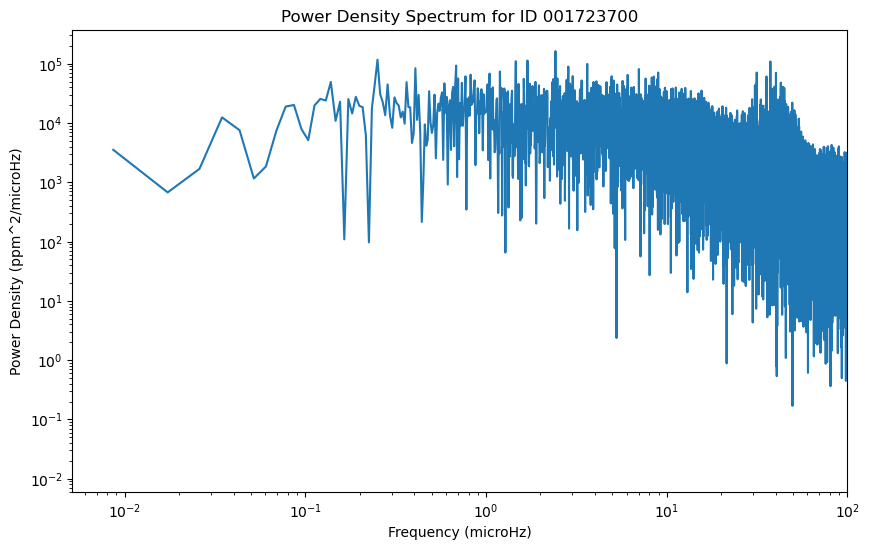
\includegraphics[width=\linewidth]{pds.png}
  \caption{Power spectrum density of a star observed by the Kepler mission}
  \label{fig:pds}
\end{figure}

\subsection{Oscillation spectrum}
The power spectrum density is a super-composition of stellar background, noise and oscillation spectrum. The region on the power spectrum density where the oscillations modes dominate over the noise is called the power excess. This region can be modelled by Gaussian envelope centered on the frequency of the maximum power, $\nu_{max}$.  

% \begin{equation}
%     f(\nu) = Aexp(\frac{(\nu - \nu_{max})^2}{2\sigma^2})
% \end{equation}

% where 
% \begin{itemize}
%     \item A is the amplitude (height) of the Gaussian 
%     \item $\sigma$ is the standard deviation which indicates the width of the Gaussian.
% \end{itemize}

Stellar background (oscillations coming from the granulation on the surface of the Sun) can be approximated by a power law resulting in a local mean background, $B(\nu)$, around $\nu_{max}$. These all were put into following model:

% \begin{equation}
%     B(\nu) = B_{max}(\nu_{max})(\frac{\nu}{\nu_{max}})^\beta
% \end{equation}

% where 
% \begin{itemize}
%     \item $B_{max}(\nu_{max})$ is background at frequency of maximum power $\nu_{max}$
%     \item $\beta$ is an exponent factor.
% \end{itemize}

% The power density spectrum model was then approximated as the sum of the background, $B(\nu)$, power excess, $f(\nu)$, and constant photon noise, $\sigma_{photon}$ as follows:

% \begin{equation}
%    M_{PE}(\nu) = f(\nu) + B(\nu) + \sigma_{photon} 
% \end{equation}

\subsubsection*{Power Spectrum Model for the background fit}
The power spectrum model combines a background term, a power excess (Gaussian envelope), and constant photon noise:

\begin{equation}
    P_{\text{model}}(\nu) = P_{\text{background}}(\nu) + P_{\text{Gaussian}}(\nu) + P_{\text{photon}}
\end{equation}

where:
\begin{itemize}
    \item \textbf{Stellar Background Term (power law):}
    \begin{equation}
        P_{\text{background}}(\nu) = B_{\nu_{\text{max}}} \left( \frac{\nu}{\nu_{\text{max}}} \right)^{\beta}
    \end{equation}
    with:
    \begin{itemize}
        \item $B_{\nu_{\text{max}}}$: Scaling factor for the background power which is background function at frequency of maximum power $\nu_{max}$.
        \item $\beta$: Spectral slope.
        \item $\nu_{\text{max}}$: Frequency of maximum power.
    \end{itemize}

    \item \textbf{Excess Power (Gaussian Peak):}
    \begin{equation}
        P_{\text{Gaussian}}(\nu) = A \exp\left(-\frac{1}{2} \left( \frac{\nu - \nu_{\text{max}}}{\sigma} \right)^2 \right)
    \end{equation}
    with:
    \begin{itemize}
        \item $A$: Amplitude of the Gaussian peak.
        \item $\nu_{\text{max}}$: Frequency of maximum power = Central frequency of the peak.
        \item $\sigma$: Standard deviation (width) of the peak.
    \end{itemize}

    \item \textbf{Photon Noise:}
    \[
    P_{\text{photon}}.
    \]
\end{itemize}

Thus:
\begin{equation}\label{eq:modelP}
    P_{\text{model}}(\nu) = B_{\nu_{\text{max}}} \left( \frac{\nu}{\nu_{\text{max}}} \right)^{\beta} + A \exp\left(-\frac{1}{2} \left( \frac{\nu - \nu_{\text{max}}}{\sigma} \right)^2 \right) + P_{\text{photon}}.
\end{equation}

The model (equation \ref{eq:modelP}) was fitted to the observations using MCMC with algorithm as mentioned in the Introduction section. 
Six parameters used in a fit are displayed in Table \ref{tab:MCMC_param}. Prior probability ranges were adjusted in the process of finding the best fit with help of corner plots (see the corner plot for MCMC fit of PSD in Appendix \ref{a:A} (Figure \ref{fig:corner_powerExcess})). The ranges were adjusted in a way to encapsulated the converged normal posterior distribution. The fit plotted with respect to its component and observed data can be seen in Figure \ref{fig:fit_powerExcess}. We found the frequency of the maximum power to be $\nu_{max} = 38.15_{-0.34}^{+0.30} \mu Hz$.

\begin{table}[H]
  \centering
  \begin{tabular}{|c|c|c|c|c|}
    \hline 
    & & & &\\[-0.5em]
    Param. Name & Code Name & Initial Guess & Prior Distr. Range & The best fit value \\[5pt] \hline
    & & & &\\[-0.5em]
    $B_{max}(\nu_{max})$ & \texttt{b\_nu\_max} & 1573.04$^*$ & [0, 1e6] & $606.64_{-29.39}^{+30.68}$ \\[5pt] \hline
    & & & &\\[-0.5em]
    $\beta$ & \texttt{beta} & -1.51$^*$ & [-3, -1] & $-2.24_{-0.05}^{+0.05}$\\[5pt] \hline
    & & & &\\[-0.5em] 
    A & \texttt{A} & 1e4 & [0, 1e6] & $3480.68_{-103.57}^{+120.22}$\\[5pt] \hline
    & & & &\\[-0.5em]
    \textbf{$\nu_{max}$} & \textbf{\texttt{nu\_max}} & \textbf{39.23$^*$} & \textbf{[35, 45]} & $38.15_{-0.34}^{+0.30}$\\[5pt] \hline 
    & & & &\\[-0.5em]
    $\sigma$ & \texttt{sigma} & 5 & [0, 10] & $8.54_{-0.23}^{+0.29}$\\[5pt]  \hline
    & & & &\\[-0.5em]
    $\sigma_{photon}$ & \texttt{P\_photon} & 1e2 & [0, 1e3] & $456.80_{-3.87}^{+4.52}$\\[5pt] \hline
  \end{tabular}
  \caption{Parameters for the MCMC fitting of background and power excess. The initial guesses where found by simple analysis of the PSD zoomed in on excess power (except $^*$, where the values were given in the text data file). The second to last column represents the uniform prior probability of parameters. The last column is the best fit value from the MCMC fit.}
  \label{tab:MCMC_param}
\end{table}

\begin{figure}[H]
  \centering
  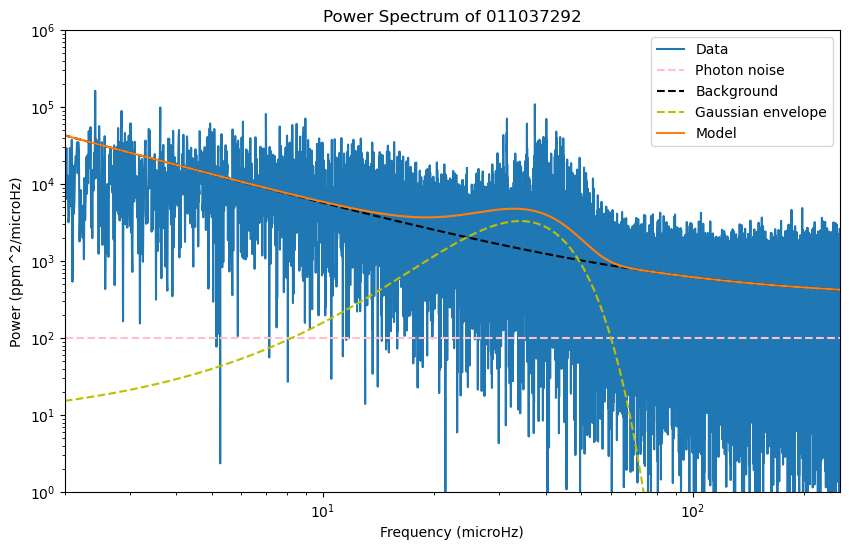
\includegraphics[width=\linewidth]{fit_powerExcess.png}
  \caption{Fit of the global power density spectrum. The pink dashed line is
a photon noise, the yellow dashed line is approximation of the local background and the dark dashed line corresponds to the oscillation excess power. The sum of these three components gives the fit of the PSD in orange solid line.}
  \label{fig:fit_powerExcess}
\end{figure}

\subsubsection*{Log-Likelihood in the Provided Code}
In the provided code, the log-likelihood is defined as:
\[
\mathcal{L}(\boldsymbol{\theta}) = - \sum_i \left[ \ln M(\nu_i, \boldsymbol{\theta}) + \frac{P_{\text{obs},i}}{M(\nu_i, \boldsymbol{\theta})} \right],
\]
where:
\begin{itemize}
    \item $M(\nu_i, \boldsymbol{\theta})$: The model power spectrum at frequency $\nu_i$ with parameters $\boldsymbol{\theta}$.
    \item $P_{\text{obs},i}$: The observed power density at $\nu_i$.
\end{itemize}

This expression penalizes discrepancies between the observed and modeled power spectrum:
\begin{itemize}
    \item The term $\ln M(\nu_i, \boldsymbol{\theta})$ reflects the logarithmic likelihood of the model.
    \item The term $\frac{P_{\text{obs},i}}{M(\nu_i, \boldsymbol{\theta})}$ penalizes mismatches between the observed and modeled values.
\end{itemize}


\subsection{Radial pressure modes}
In order to isolate the oscillations spectrum, we subtracted the background and noise from the PSD (see the results zoomed in our region of interest around $\nu_{max}$ in Figure \ref{fig:wB}). We performed fit of pure radial pressure modes using the Lorentzian model: 

\begin{figure}[H]
  \centering
  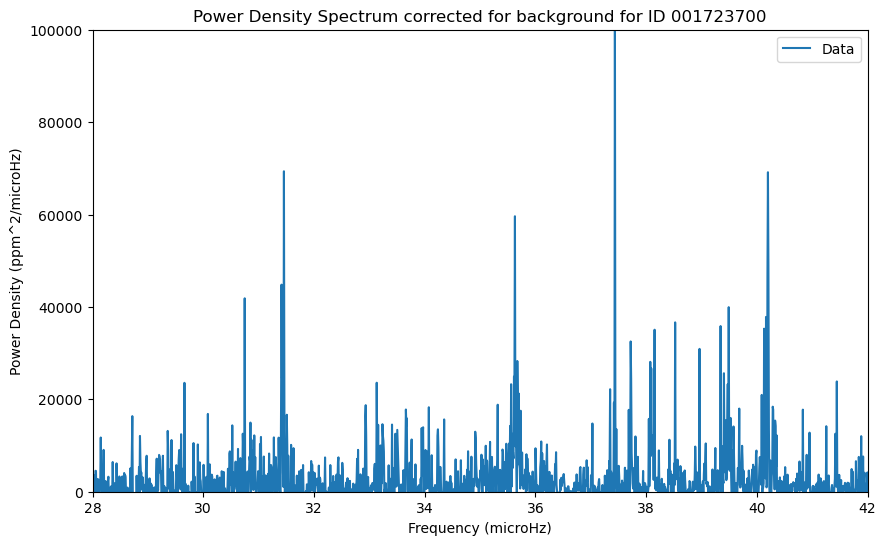
\includegraphics[width=\linewidth]{withoutB.png}
  \caption{Power spectrum density after a subtraction of background zoomed in our region of further interest.}
  \label{fig:wB}
\end{figure}

\subsubsection*{Lorentzian Model}
The Lorentzian model represents the sum of two Lorentzian functions at different frequency centers (we dropped $m$ in each equations as we considered it to be 0):

\begin{equation}\label{eq:Lmodel}
  L_{\text{model}}(\nu) = \sum_n \sum_{l_0}^{l_{max}} L_{n,l}(\nu)  
\end{equation}

where each Lorentzian is defined as:
\begin{equation}
    L_{n,l}(\nu) = \frac{H_{n,l}}{1 + 4 \left( \frac{\nu - \nu_{\text{center},n,l}}{\Gamma_{n,l}} \right)^2}
\end{equation}

where
\begin{itemize}
    \item $H_{n,l}$ is height of the Lorentzian peak.
    \item $\Gamma_{n,l}$ is line-width of the Lorentzian peak (half width at half-maximum).
    \item $\nu_{\text{center},n,l}$ is a central frequency of the peak.
\end{itemize}

Central frequency of the peak is defined as 
\begin{equation}
    \nu_{\text{center},n,l} = \left( n + \frac{l}{2} + \epsilon + d_{0l} + \frac{\alpha}{2} (n - n_{\text{max}})^2 \right) \Delta\nu
\end{equation}

where:
    \begin{itemize}
        \item $n_{\text{max}} = \frac{\nu_{\text{max}}}{\Delta\nu} - \epsilon$ is a central radial order.
        \item $\Delta\nu$ is a large frequency spacing.
        \item $\epsilon$ is a phase constant.
        \item $\alpha$ is the curvature term on $\Delta\nu$.
    \end{itemize}


The radial order $n$ have to be considered around the value $n_{max}$ in equation \ref{eq:Lmodel} and only degrees $l < l_{max} = 3$ are present in oscillation spectra obtained by photometric observations.

At first, we determine the $n_{max}$ with $\epsilon$, $\Delta\nu$ and $\nu_{max}$ to be $n_{max} = 7.54$. As this is not integer, we took our radial order to be $n=8$ (we also tried $n=7$ but the fit was unsuccessful). We fit for angular degrees $l=0,1,2$. However, the fit was not successful with $l=1$. This mode $L_{8,1}$ could not be resolved and hence it was excluded from out final fit and was not used in further analysis as well. Parameters used in a fit are displayed in Table \ref{tab:MCMC_param_lorentz}, 5 of the parameters were free while others were kept constant ($\epsilon$, $\Delta\nu$ and $\nu_{max}$ were assumed to be constant). Prior probability ranges were adjusted in the process of finding the best fit with help of corner plots (see the corner plot for MCMC Lorentzian fit of pressure modes in Appendix \ref{a:B} or Figure \ref{fig:corner_lorentz1}). The ranges were adjusted in a way to encapsulated the converged normal posterior distribution. The Lorentzian fit plotted with respect to the observed pressure modes can be seen in Figure \ref{fig:fit_pressureMode1}.

% \begin{itemize}
%     \item \textbf{For the first Lorentzian ($L_1$):}
%     \[
%     \nu_{\text{center},1} = \left( n + \frac{0}{2} + \epsilon + 0 + \frac{\alpha}{2} (n - n_{\text{max}})^2 \right) \Delta\nu,
%     \]
%     where:
%     \begin{itemize}
%         \item $n_{\text{max}} = \frac{\nu_{\text{max}}}{\Delta\nu} - \epsilon$: Central radial order.
%         \item $\Delta\nu$: Large frequency spacing.
%         \item $\epsilon$ is a phase constant.
%         \item $\alpha$ is the curvature term on $\Delta\nu$.
%     \end{itemize}

%   \item \textbf{For the second Lorentzian ($L_2$):}
%     \[
%     \nu_{\text{center},2} = \left( n - 1 + \frac{2}{2} + \epsilon + d_{0l} + \frac{\alpha}{2} (n - 1 - n_{\text{max}})^2 \right) \Delta\nu,
%     \]
%     where:
%     \begin{itemize}
%         \item $d_{0l}$: Small frequency spacing parameter.
%     \end{itemize}
% \end{itemize}

% Thus:
% \[
% L_{\text{model}}(\nu) = \frac{H_1}{1 + 4 \left( \frac{\nu - \nu_{\text{center},1}}{\Gamma_1} \right)^2} + \frac{H_2}{1 + 4 \left( \frac{\nu - \nu_{\text{center},2}}{\Gamma_2} \right)^2}.
% \]

\begin{table}[H]
  \centering
  \begin{tabular}{|c|c|c|c|c|}
    \hline 
    & & & &\\[-0.5em]
    Param. Name & Code Name & Initial Guess & Prior Distr. Range & The best fit value \\[5pt] \hline
    & & & &\\[-0.5em]
    $H_{8,0} $ & \texttt{H1} & 5e4 & [1e4, 6e4] & $25613.70$ \\[5pt] \hline
    & & & &\\[-0.5em]
    $H_{8,2}$ & \texttt{H2} & 2e4 & [1e2, 4e4] & $8719.84$\\[5pt] \hline
    & & & &\\[-0.5em] 
    $\Gamma_{8,0}$ & \texttt{Gamma1} & 0.25 & [0.01, 1] & $0.14$\\[5pt] \hline
    & & & &\\[-0.5em]
    $\Gamma_{8,2}$ & \texttt{Gamma2} & 0.25 & [0.01, 1] & $0.47$\\[5pt] \hline 
    & & & &\\[-0.5em]
    $d_{0l}$ & \texttt{d\_0l} & -0.15 & [-1, -0.01] & $-0.16$\\[5pt]  \hline
    & & & &\\[-0.5em]
    $\epsilon$ & \texttt{eps} & 0.961 & constant & $-$\\[5pt]  \hline
    & & & &\\[-0.5em]
    $\alpha$ & \texttt{alpha} & 0.0098 & constant & $-$\\[5pt]  \hline
    & & & &\\[-0.5em]
    $\Delta\nu$ & \texttt{delta\_nu} & 4.483 & constant & $-$\\[5pt]  \hline
  \end{tabular}
  \caption{Parameters for the MCMC fitting of Lorentzian fit to pressure modes. The initial guesses where found by simple analysis pressure modes. The second to last column represents the uniform prior probability of parameters. The last column is the best fit value from the MCMC fit. The constant values were given in data file. To see the uncertainty on the fitted parameters, see corner plot in Appendix \ref{a:B}}
  \label{tab:MCMC_param_lorentz}
\end{table}

\begin{figure}[H]
  \centering
  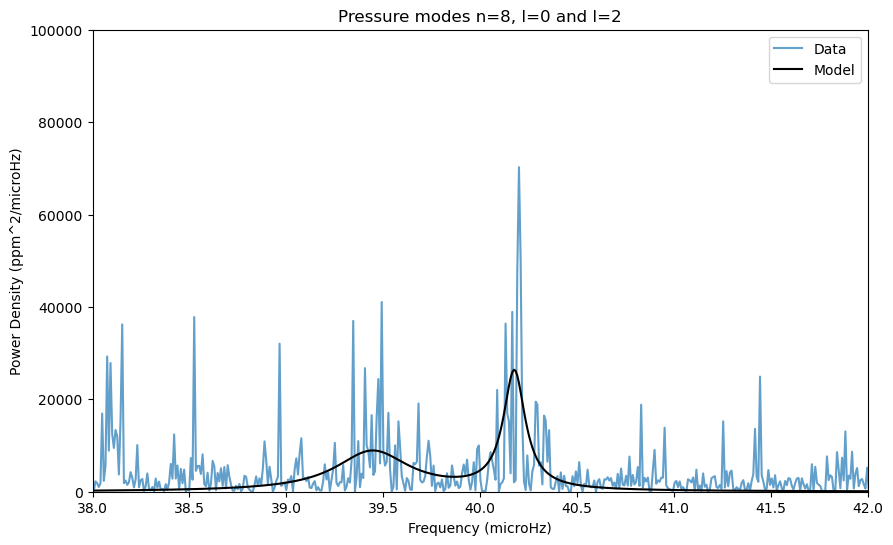
\includegraphics[width=\linewidth]{mode1.png}
  \caption{Fit of the pressure mode with radial order n=8 and angular degree l=0 and l=2. Pressure mode $L_{8,0}$ is the higher peak.}
  \label{fig:fit_pressureMode1}
\end{figure}

To get the value of the $\Delta\nu$, we fitted another radial orders ($n=7,8$), each for $l=0,2$. In this case, we have assumed only $\alpha$ to be constant (taken from the data file) and we had 10 free parameters. This doubled the free parameters, hence, the parameters, initial guesses, priors and results can be found in the appendix \ref{a:C}. We obtained $\Delta\nu = 4.57\pm 0.03 \mu Hz$. The Lorentzian fit plotted with respect to the observed pressure modes can be seen in Figure \ref{fig:fit_pressureMode2}.

\begin{figure}[H]
  \centering
  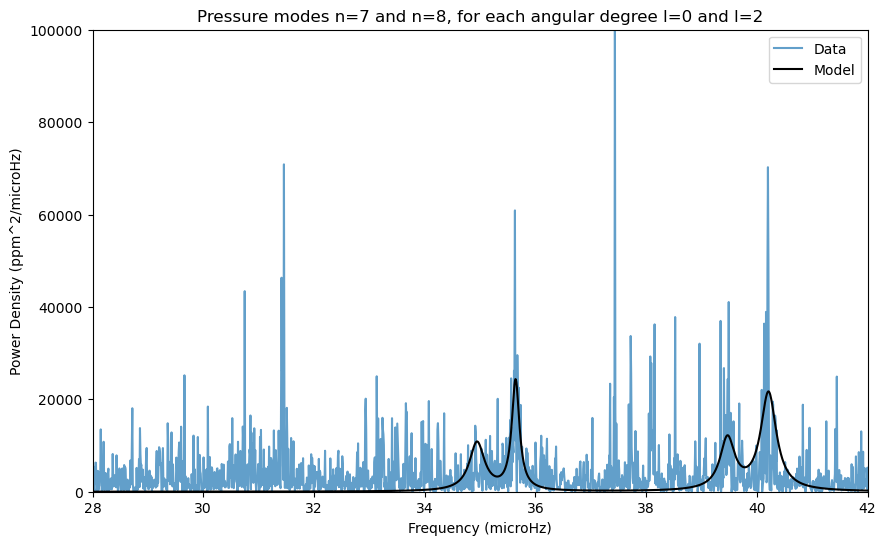
\includegraphics[width=\linewidth]{mode2.png}
  \caption{Fit of the pressure mode with radial order n=7 and n=8 and angular degree l=0 and l=2. Pressure mode $L_{8,0}$ is the higher peak on the right. Pressure mode $L_{7,0}$ is the higher peak on the left radial mode.}
  \label{fig:fit_pressureMode2}
\end{figure}

Then, we fitted the three pressure modes of radial degree $n=6,7,8$ and for each radial degree, two angular degrees $l=0,2$. Here, we kept constant $\nu_{max} = 38.1443\mu Hz$ and we have 22 free parameters which increased the computational time significantly. We found $\alpha = 0.03\pm 0.004$ and $\Delta\nu = 4.48 \pm 0.01 \mu Hz$. The final fit can be found in Figure \ref{fig:fit_pressureMode3}. The corner plot is under appendix \ref{a:D} (or Figure \ref{fig:corner_lorentz}).


\begin{figure}[H]
  \centering
  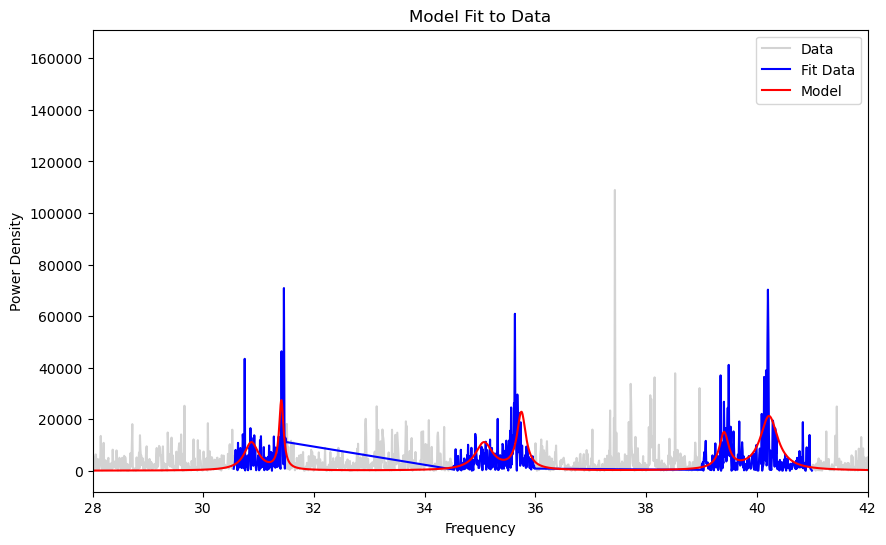
\includegraphics[width=\linewidth]{mode3.png}
  \caption{Fit of the pressure modes with radial order n=6,7,8 and angular degree l=0 and l=2 (in red). In blue are the ranges of interest containing the pressure modes, in gray the data. Radial order are from left to right increasing (6, 7, 8). In the radial orders the higher peaks are l=0, lower height l=2. The frequency position difference of successive maximum peaks is $\Delta\nu$}
  \label{fig:fit_pressureMode3}
\end{figure}

The formulas we have used here to fit the parameters are taken from the note on Seismic Analysis \cite{Benoit}; provide in the Data Analysis Master class.
\printbibliography
\appendix
\renewcommand{\thesection}{\Alph{section}}

\section{Corner plot for one radial order}\label{a:A}
\begin{figure}[H]
  \centering
  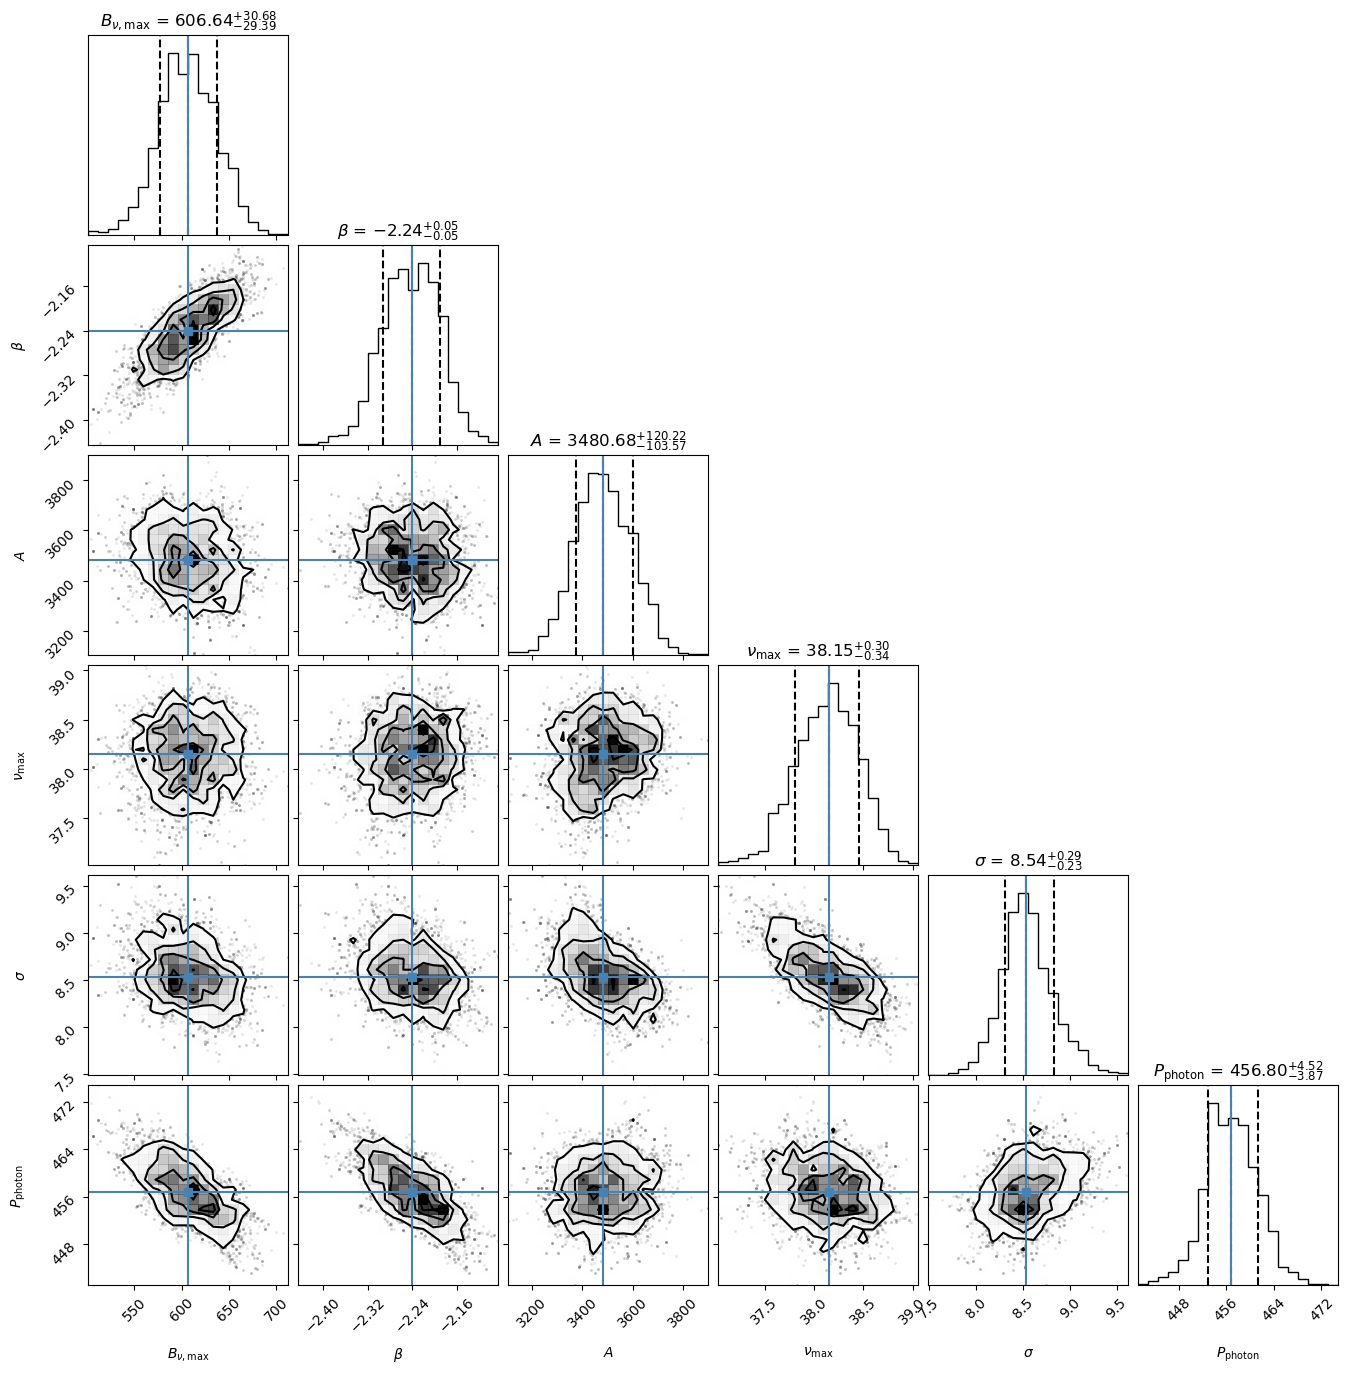
\includegraphics[width=\linewidth]{corner_pds.png}
  \caption{Corner plot displaying the posterior distributions of fitted parameters}
  \label{fig:corner_powerExcess}
\end{figure}

\newpage
\section{Corner plot for singel radial order}\label{a:B}
\begin{figure}[H]
  \centering
  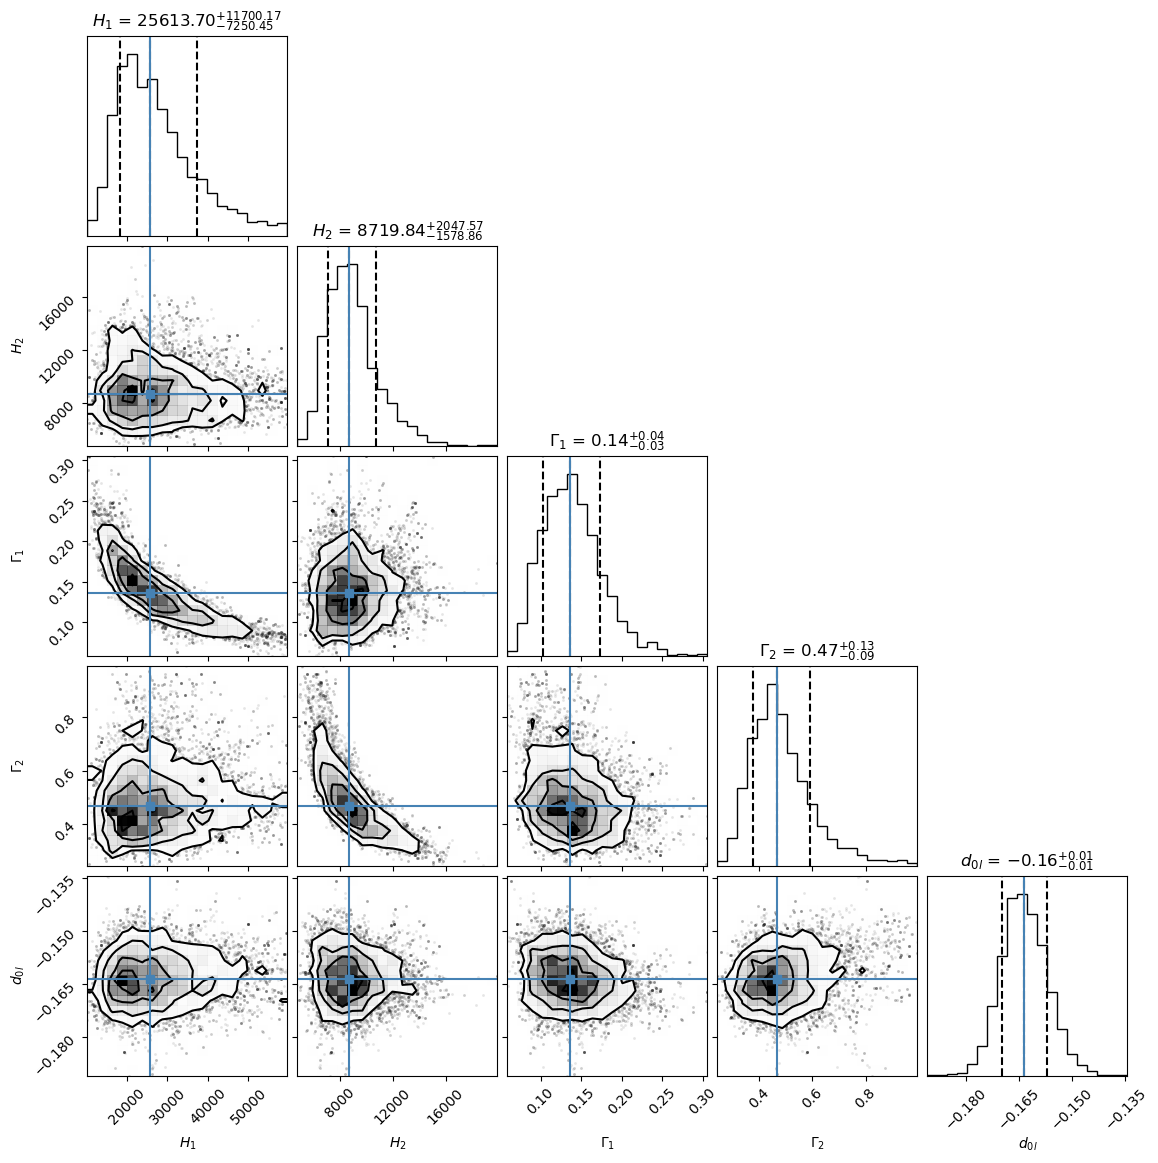
\includegraphics[width=\linewidth]{corner_lorentz1.png}
  \caption{Corner plot displaying the posterior distributions of fitted parameters. Here $H_1$, $\Gamma_1$ corresponds to $H_{n,l} = H_{8,0}$, $\Gamma_{8,0}$ and $H_2$, $\Gamma_2$ corresponds to $H_{n,l} = H_{8,2}$, $\Gamma_{8,2}$}
  \label{fig:corner_lorentz1}
\end{figure}
\newpage
\section{Corner plot for two radial orders}\label{a:C}
\begin{figure}[H]
  \centering
  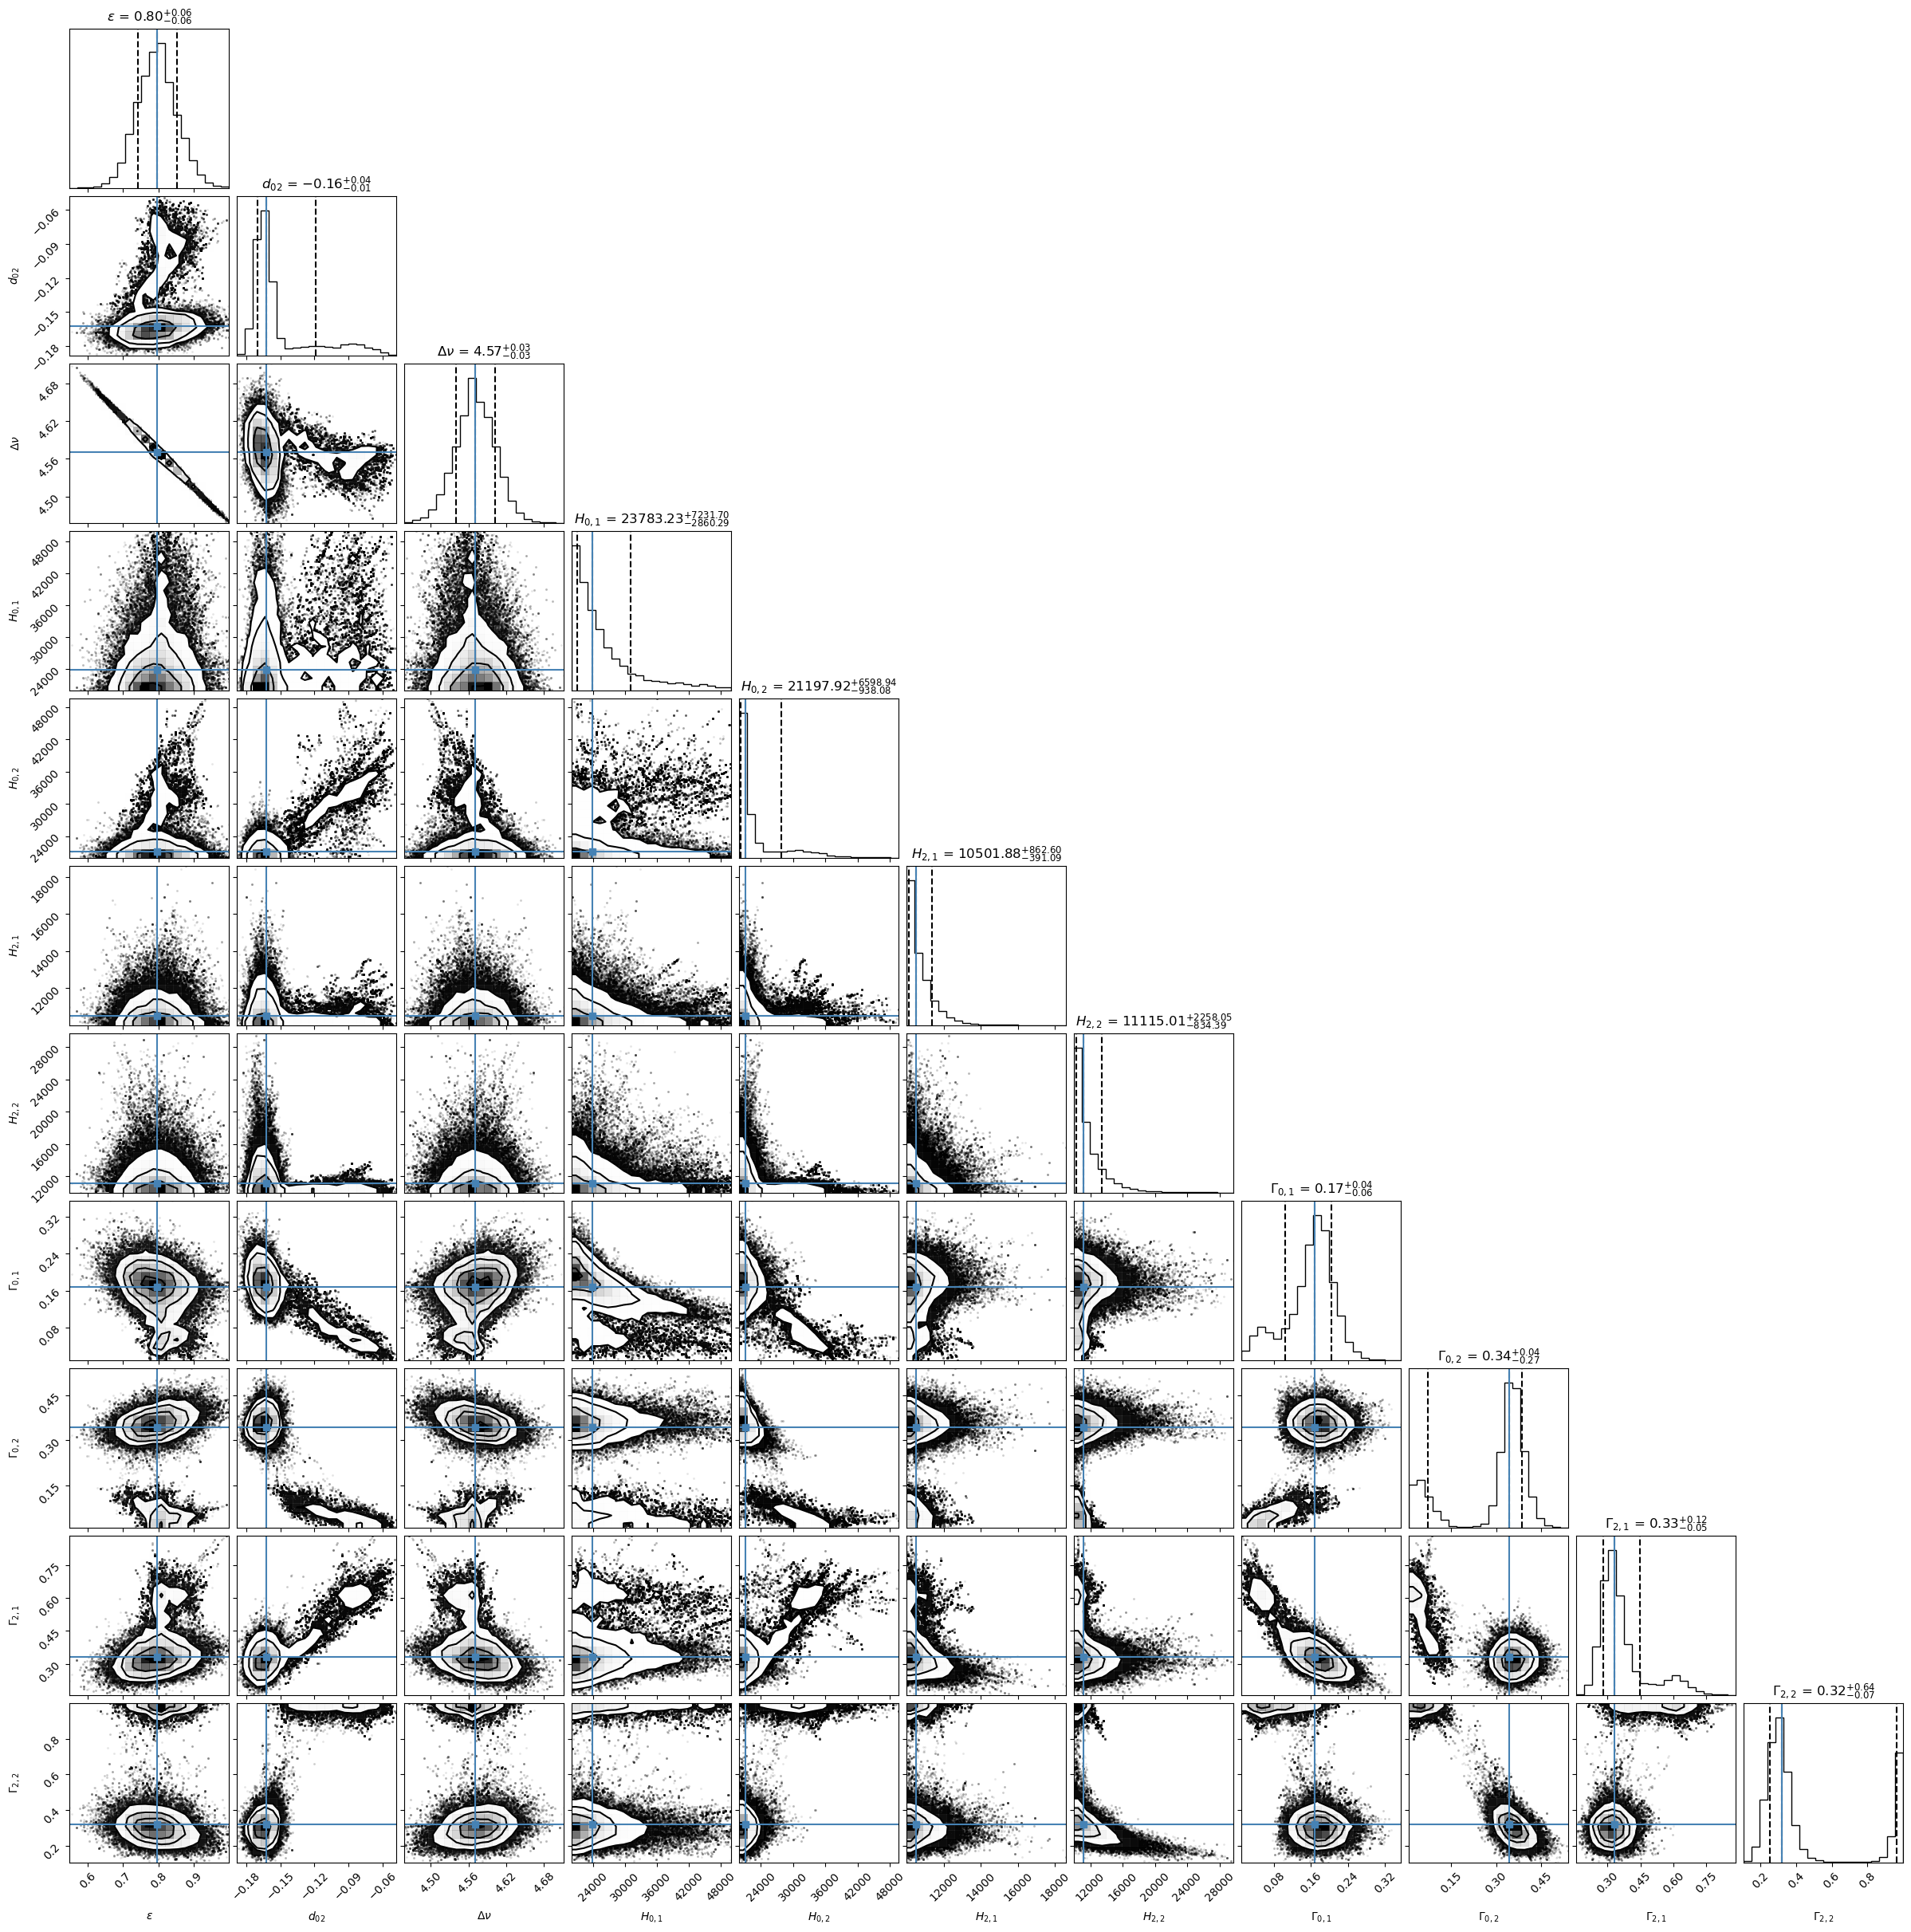
\includegraphics[width=\linewidth]{corner_lorentz2.png}
  \caption{Corner plot displaying the posterior distributions of fitted parameters. Here the first index 0,1 are for n=7,8 and the second index 0,1 are l=0,2.}
  \label{fig:corner_lorentz2}
\end{figure}
\newpage 
\section{Corner plot for three radial orders}\label{a:D}
\begin{figure}[H]
  \centering
  \includegraphics[width=\linewidth]{corner_lorentz.png}
  \caption{Corner plot displaying the posterior distributions of fitted parameters. Here the first index 0,1,2 are for n=6,7,8 and the second index 0,1 are l=0,2.}
  \label{fig:corner_lorentz}
\end{figure}
% \section{Code for star 1 (spec_001723700)}
% \input{AstroSys.pdf}
% \section{Code for star 1 (spec_006852836)}
% \input{AstroSys_star2.pdf}


\end{document}










